\documentclass[dvipdfmx,fleqn]{beamer}
%\documentclass[dvipdfmx,fleqn,handout]{beamer}
\usepackage{amsmath,amssymb,amsthm}

\mode<presentation>
{
  \usetheme{default}
}

\title{\Large Fictitious play}
\author{\large 三ツ國  拓真}
\date{\small 2014/6/30}

\usefonttheme{professionalfonts}

\setbeamercovered{transparent=20}

\setbeamertemplate{navigation symbols}{} 
\setbeamertemplate{footline}[frame number] 



\begin{document}

\sffamily
\gtfamily


\begin{frame}
  \titlepage
  \thispagestyle{empty}
\end{frame}

\setcounter{framenumber}{0}




\begin{frame}
\frametitle{はじめに}
\begin{itemize}\setlength{\parskip}{0.5em}
\item
Fictitious Playについて
(Matching Pennies を例として)

\item
シュミレーションプログラムのコードについての説明
 \begin{itemize}\setlength{\parskip}{0.5em}
 \item
 工夫した点
 \item
 今後の課題
 
\end{itemize}
\end{frame}



\begin{frame}
\frametitle{Ficititious play}
\begin{itemize}\setlength{\parskip}{0.5em}
\item
戦略形ゲームが$t=1,2,...$の各期にプレイされる。
各プレイヤーは$t+1$期に、他プレイヤーが1期からt期において選択した行動の比率に応じた確率で$t+1$期の行動をとると予想し、自分の期待利得が最大になるような行動をとる。\pause


\item
予測に対する最適反応戦略をとるモデル。
 \pause

\end{itemize}
\end{frame}




\begin{frame}
\frametitle{Matching Pennies ゲームの例}
\begin{itemize}\setlength{\parskip}{0.5em}
\item

プレイヤーは0と1の2人
行動は行動 0と行動 1 の2通り
利得は (1,-1),(-1,1)
      (-1,1),(1,-1) 

\item
$t$期にプレイヤー$i$が選択した行動は$a_i(t)$と表す
$t$期にプレイヤー$i$が持っている「信念」は$x_i(t)$と表す
 \pause
 
$x_0(t)$ は
\[
x_0(t+1)
= x_0(t) + \frac{1}{t+2} (a_1(t) - x_0(t))
\]
と再帰的に書くことができる. \pause

\item
プレイヤー 0 の行動の決め方  (プレイヤー 1 についても同様.)
「プレイヤー 1 は,確率 $1−x_0(t)$ で行動 0 をとり,確率 $x_0(t)$ で行動 1 をとる」 と考え,自分の期待利得が最大になるような行動をとる(行動 0,1 の期待利得が等しい場合は確率半々でランダムに選ぶ)
行動は信念に依存して決定される
 \pause

\item
プレイヤー 0 の信念の決まり方  (プレイヤー 1 についても同様.)
初期信念 $x_0(0)$ は [0,1] 上の一様分布にしたがってランダムに与えられる.
 \item
 各$t\geq1$期において、プレイヤー1が過去とった行動を$a_1(0),...,a_1(t-1)$とすると、
 信念$x_0(t)$は、
 \[
 x_0(t)
 = \frac{x_0(0)+a_1(0)+...+a_1(t-1)}{t+1} 
 \]
 で与えられる。
 \item
 これは、
 \[
 x_0(t+1)
 = x_0(t) + \frac{1}{t+2} (a_1(t) - x_0(t))
 \]
 と再帰的に書くことができる。 \pause

\item
このように信念は自らの初期信念と相手の過去の行動に依存して決まる。

\end{itemize}
\end{frame}






\begin{frame}[fragile]% verbatim 環境を使えるように
\frametitle{コード}
\begin{itemize}\setlength{\parskip}{0.5em}
\item
コード
\begin{verbatim}
import numpy as np
import matplotlib.pyplot as plt
import pylab as pl
from random import uniform

p = [[1,-1], [-1, 1], [-1,1], [1, -1]]    #利得


        
def Fictplay(n):
    x0 = [uniform(0, 1)] #初期信念をランダムに設定,appendを使い後に更新する
    x1 = [uniform(0, 1)]
    
    for t in range(n):
            #期待利得 
        ep0 = [p[0][0]*(1-x0[t])+p[1][0]*x0[t], p[2][0]*(1-x0[t])+p[3][0]*x0[t]]
        ep1 = [p[0][1]*(1-x1[t])+p[2][1]*x1[t], p[1][1]*(1-x1[t])+p[3][1]*x1[t]]
            
            #期待値の大きくなる行動を選択
        if ep0[0] > ep0[1]:
                a0 = 0
        else:
                a0 = 1
        if ep1[0] > ep1[1]:
                a1 = 0
        else:
                a1 = 1
            # append
        x0.append(x0[t]+(a1-x0[t])/(t+2))   ##i+1期の信念を計算
        x1.append(x1[t] +(a0-x1[t])/(t+2))
    return x0, x1

x0, x1 = Fictplay(10000)   #t=10000までの信念の推移

            

plt.plot(x0, 'r-', label = 'x0(t)')
plt.plot(x1, 'b-', label = 'x1(t)')
plt.show()

x0_last = []
for i in range(100):    #Fictplay(10000)を100回繰り返し最後の信念をヒストグラム化
    x0, x1 = Fictplay(10000)
    x0_last.append(x0[9999])
plt.hist(x0_last)
plt.show()
\end{verbatim}

\item

\end{itemize}
\end{frame}



\begin{frame}
\frametitle{図}
\begin{figure}
 \centering
 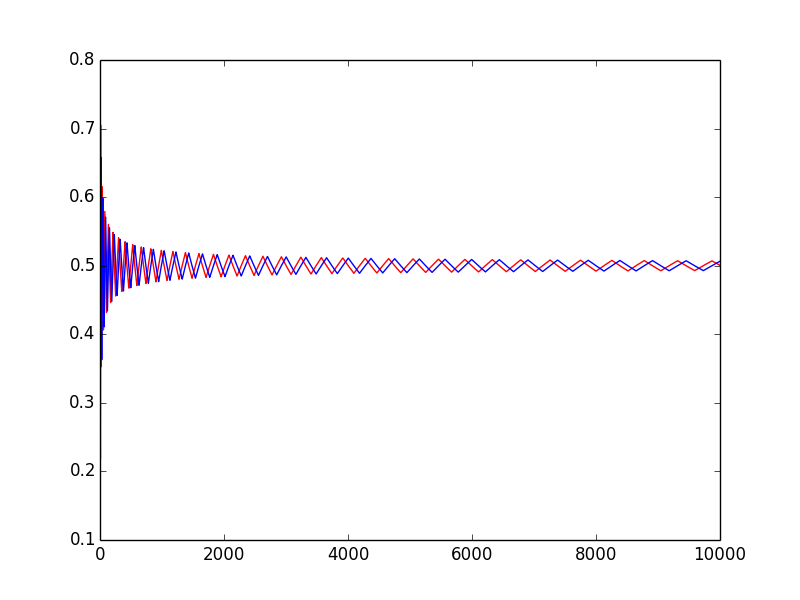
\includegraphics{fictplay.pdf}
 \caption{t=10000のときの信念の推移}
 \label{fig:matchingpennies_plot}
\end{figure}
\end{frame}



\begin{frame}
\frametitle{まとめ}
\begin{itemize}\setlength{\parskip}{0.5em}
\item
回数を重ねるごとに$0.5$に収束しているようである。



\item
classで定義してみる。
利得の行列表記をやってみる。
コーディネーションゲームなど他のゲームのシミュレーションをやってみる。
\end{itemize}
\end{frame}



\end{document}